% Dissertation LaTeX Template
% Author: Karol Cieslik
% LinkedIn: https://www.linkedin.com/in/karolcieslik/
% I have developed this template over the years.
% I hope that it will be useful for others. 
% It works both for thesis in English and in Polish.

\documentclass[11pt,twoside]{report}
\usepackage[left=35mm,top=25mm,right=25mm,bottom=25mm]{geometry}
\usepackage{indentfirst}
\usepackage{polski}
\usepackage[polish,english]{babel}
\usepackage{amsmath} % Required for some math elements 
\usepackage[titletoc]{appendix}
\usepackage{rotating} 
\usepackage[
protrusion=true,
activate={true,nocompatibility},
final,
tracking=true,
kerning=true,
spacing=true,
factor=1100]{microtype}
\SetTracking{encoding={*}, shape=sc}{40}
\newsavebox{\myhbar}
\savebox{\myhbar}{$\hbar$}
\renewcommand*{\hbar}{\mathalpha{\usebox{\myhbar}}}
\usepackage[utf8]{inputenc}
\usepackage[version=3]{mhchem} % Package for chemical equation typesetting
\usepackage{siunitx} % Provides the \SI{}{} and \si{} command for typesetting SI units
\usepackage{graphicx} % Required for the inclusion of images
\usepackage{float}
\usepackage{wrapfig}
\usepackage{fancyhdr} % Custom headers and footers
\pagestyle{fancyplain} % Makes all pages in the document conform to the custom headers and footers
\setlength\parindent{0.75cm}
\linespread{1.15}
\fancyhf{} 
\fancyfoot[R]{\thepage}
\pagestyle{fancy}
\fancyhead[L]{\scshape\nouppercase{\rightmark}}
\setlength{\headheight}{13pt} 
\usepackage{titlesec}
 \titleformat{\chapter}[display]   
{\normalfont\huge\bfseries}{\chaptertitlename\ \thechapter}{20pt}{\Huge}   
\titlespacing*{\chapter}{0pt}{-20pt}{20pt}
\usepackage{caption}
\usepackage[font={small}]{caption}
\usepackage{enumerate}
\usepackage{multirow}
 \graphicspath{{wykresy/}}
   \usepackage[unicode=true]{hyperref}
\renewcommand\refname{Bibliografia}
\newcommand{\horrule}[1]{\rule{\linewidth}{#1}} 

% In the SI package you can declare your own units which comes in handy
\DeclareSIUnit{\ions}{ions} 
\DeclareSIUnit{\langmuir}{L} 



\usepackage{hypcap}
\usepackage{booktabs}
\newcommand\doubleRule{\toprule\toprule}
\newcommand\doublerule{\toprule\specialrule{\heavyrulewidth}{\doublerulesep}{0.4em}}
\newcommand{\ra}[1]{\renewcommand{\arraystretch}{#1}}
\AtBeginDocument{\addtocontents{toc}{\protect\thispagestyle{empty}}}
\usepackage{emptypage}
\usepackage{etoolbox}
\patchcmd{\chapter}{plain}{plain}{}{}
\usepackage{hyperref}
\setlength{\belowcaptionskip}{-10pt}
\usepackage{enumitem}
\setlist[itemize]{noitemsep, topsep=0pt}
\usepackage{booktabs,caption}
\usepackage[flushleft]{threeparttable}
\usepackage{acronym} 

%this package is just useful for the template 

\usepackage{lipsum}  

\begin{document}
	\begin{titlepage}
	\centering
	%\vspace*{1cm}
	\Large
	\textsc{University Name \\ The name of the Institute \\ Department of Something or Other} \\ \vspace*{1\baselineskip}
	
	
\includegraphics[width=0.25\textwidth,height=0.25\textheight,keepaspectratio]{uj_logo.jpg}
	
	\horrule{0.5pt} \\[0.4cm] % Thin top horizontal rule
	\Huge  The title of your thesis. Encompassing everything you have done in a short and interesting way. \\ 
	\horrule{2pt} \\[0.5cm] % Thick bottom horizontal rule
	
	\Large{Doctoral thesis \\ \textit{submitted by}}
	\vspace*{1\baselineskip}
	
	\LARGE \textbf{Name Surname} \\
		\vspace*{1\baselineskip}

	\Large{\textit{supervised by:} \\ prof. Name Surname \\}
		
	\vspace*{2\baselineskip}
	\Large{City, Year}
	
    \end{titlepage}
\shipout\null
\newpage
\thispagestyle{empty}
\vspace*{30px}
\begin{flushleft}
\large{Department Name\\
University name}
\end{flushleft}
\vspace*{1\baselineskip}


\hspace{5.31cm}{\textbf{\Large{Declaration}}

\vspace*{15px}

{\large{\lipsum[5]

\lipsum[12]

\vspace*{25px}
\begin{center}
	\begin{tabular}{lr}
		................................~~~~~~~~~~~~~~~~~~~~~~~~~~~~~~~~~~~~~~&
		.......................................... \\
		{~~~~~~~~City, date} & {Your signature~~~~~~~}
	\end{tabular}
\end{center}
\noindent \hfill 


\noindent  \hfill }}}
\\

%the numbering should be different in the sections before the main body of the dissertation


\pagenumbering{roman}
\setcounter{page}{0}

\clearpage
\phantomsection
\addcontentsline{toc}{chapter}{Acknowledgements}
\chapter*{Acknowledgements}

\lipsum[1-3]  
\clearpage
\phantomsection
\addcontentsline{toc}{chapter}{Acknowledgements in another language}
\include{chapters/Acknowledgements2}  
\clearpage
\phantomsection
\addcontentsline{toc}{chapter}{Abstract}
\chapter*{Abstract}

\lipsum[5-7]


  
\clearpage
\phantomsection
\addcontentsline{toc}{chapter}{Abstract in another language}
\include{chapters/Abstract2}   
\clearpage
\phantomsection
\addcontentsline{toc}{chapter}{Acronyms}
\chapter*{Acronyms}
\begin{acronym}
\acro{AES}{Auger electron spectroscopy}
\acro{AFM}{Atomic force microscopy}
\end{acronym}          

%the style of numbering of pages

\pagenumbering{arabic}

%you can add some chapters 

\tableofcontents

%you can add some chapters 

\pagenumbering{arabic}
\chapter{Introduction}


\lipsum[12]


Here you can also cite a publication. Like this \cite{Cie2022}.


\section{Thesis structure}

\lipsum[4]


\begin{itemize}
	\item Chapter 1 – \textbf{Introduction}
	
	This chapter contains a the introduction. 
	
	\item Chapter 2 – \textbf{Some nice chapter}
	
	The chapter outlines some great results.
	
	\item Chapter 3 – \textbf{Experimental}
	
	This part of the dissertation describes experimental details.

	\item Chapter 4 - \textbf{Conclusions}
	
	This chapter contains the conclusions.

	\item Appendix - \textbf{Academic achievements}
	
	The publications and conferences at which  the results were presented are listed here. 
\end{itemize}

\section{Motivations}

\lipsum[5-7]


\section{Some section with an equation and citations}


Here the Equation \ref{reaction-oxidation-sto} starts:
\begin{equation}
	k \cdot \ce{ SrTiO3} \ce{->} p \cdot \ce{ SrTiO3}  +   q \cdot \ce{SrO (SrTiO3)_n} +  q \cdot \ce{TiO2},
	\label{reaction-oxidation-sto}
\end{equation}
where $k = q\cdot (n+1) + p$. And here it ends.


\subsection{A subsection}

\lipsum[12]

\section{Some section with a figure} \label{section-with-figure}

\lipsum[15-16]
\begin{figure} [!h]
	\centering
	%\captionsetup{justification=centering}
	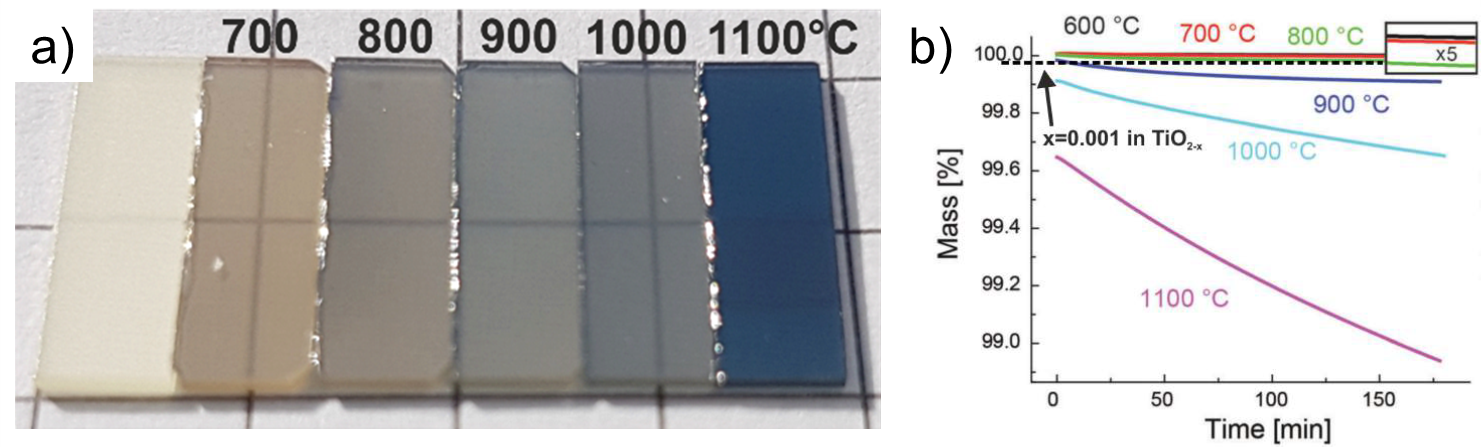
\includegraphics[width=14cm,height=8cm,keepaspectratio]{figures/introduction/annealing-intro}
	\setlength\belowcaptionskip{3pt}
	\caption{Some figure with with part a) and b).}
	\label{some-figure}
\end{figure}


We are in the Section \ref{section-with-figure} with Figure \ref{some-figure}.


\lipsum[19-20]







\chapter{Experimental}

\lipsum[7]

\section{Something about the experiment }

\lipsum[8]
 
\subsection{A subsection with a table } 

\lipsum[9-10]


\vspace{7pt}
\begin{table}[!h]
	\centering
	\ra{1.1}
	\caption{The comparison of published desorption energy and pre-exponential factor of 6P multilayer with the ones obtained from manual linear heating and passive cooling of the 6P powder. The values of kinetic parameters calculated using heating curves obtained based on different assumptions.}
	\label{arr_tab_6p}
	\vspace{-5pt}
	\resizebox{\textwidth}{!}{%
		\begin{tabular}{@{}lS[table-format=1.3]S@{}}
			\doublerule
			& {Desorption energy (\si{\electronvolt})}   & {Pre-exponential factor (\si{\per \second})}    \\
			\midrule
			Manual linear heating       & 3.54(2) & \SI{6.2(5)E33}{}   \\
			Manual linear heating  (different assumptions)      &  &    \\
			\hspace{1cm}Linear region after \SI{2}{min}, offset \SI{30}{\celsius}       & 3.93(2) & \SI{2.8(2)E35}{} \\
			\hspace{1cm}Linear region after \SI{2}{min}, offset \SI{-30}{\celsius}        & 3.18(2) &  \SI{1.4(1)E32}{} \\
			\hspace{1cm}Linear region after \SI{3}{min}, offset \SI{0}{\celsius}     & 2.84(2) & \SI{2.8(2)E27}{} \\		
			\hspace{1cm}Linear region after \SI{1}{min}, offset \SI{0}{\celsius}   & 4.10(2) & \SI{6.4(5)E38}{} \\
			Manual linear heating  (with estimated error)      & 3.5(7)  & \phantom{(0.00..)}{$6 \times 10^{33(5)}$}  \\ \midrule
			Passive cooling       & 3.17(2) & \SI{2.4\pm0.2E32}{} \\
			Passive cooling   (with estimated error)      & 3.2(2)  & \phantom{(0.00..)}{$2 \times 10^{32(1)}$}  \\ \midrule
			6P multilayer, A. Winkler (2015)    & 2.4     & \phantom{(00.)}\SI{6E25}{} \\
			\bottomrule   
	\end{tabular}}
\end{table}



\textbf{The table shows how one can use the SI package to align values in a column to a symbol or a decimal point. }



\subsection{A giant complicated table for a whole page}

\lipsum[61]


\begingroup
\renewcommand*{\arraystretch}{1.4}

\begin{sidewaystable}[]
	\centering
	\ra{1.1}	
	\caption{Summary of the used annealing methods describing their characteristics in the context of oxide reduction experiments.}
	\label{annealing-summary}
	\resizebox{\textwidth}{!}{%
		\begin{tabular}{@{}lllllll@{}}\doublerule
			Annealing method                                                          & Sample                                                            & Max temp. of sample                                                                                                                                                                     & Temp. uniformity                                                                   & Temp. of getter                                                                                                       & Cleanliness                                                                & ELOP usefulness                                                   \\ \midrule
			\begin{tabular}[c]{@{}l@{}}Current through\\ sample \\ \\ \phantom{empty}\end{tabular} & \begin{tabular}[c]{@{}l@{}}Monocrystal\\ \\ \\ \phantom{empty}\end{tabular} & \begin{tabular}[c]{@{}l@{}}Depending on type of crystals\\ and luck, for \ce{TiO2} on\\ Si \textgreater{}\SI{1350}{\degreeCelsius}, for \ce{SrTiO3} on Si \SI{1250}{\degreeCelsius}\\ was achieved\end{tabular}                          & \begin{tabular}[c]{@{}l@{}}Relatively uniform\\ below \SI{1050}{\degreeCelsius}\\ (approx. \SI{30}{\degreeCelsius})\\ \\ \phantom{empty}\end{tabular} & \begin{tabular}[c]{@{}l@{}}Unknown, but higher\\ than the studied\\ sample's*\\ \phantom{empty}\end{tabular}                                   & \begin{tabular}[c]{@{}l@{}}Clean\\ \\ \\ \phantom{empty}\end{tabular}                & \begin{tabular}[c]{@{}l@{}}Useful \\ \\ \\ \phantom{empty}\end{tabular}     \\ \hline
			\begin{tabular}[c]{@{}l@{}}Electron beam\\ holder\\ \\ \phantom{empty}\end{tabular}    & \begin{tabular}[c]{@{}l@{}}Monocrystal\\ \\ \\ \phantom{empty}\end{tabular} & \begin{tabular}[c]{@{}l@{}}Temp. of sample above \textgreater{}\SI{1350}{\degreeCelsius},\\ temperatures of \SI{1668}{\degreeCelsius}  reached\\ (melting temp of Ti), high temp\\ can be reached without difficulty\end{tabular} & \begin{tabular}[c]{@{}l@{}}Relatively uniform\\ below \SI{1050}{\degreeCelsius}\\ (approx. \SI{30}{\degreeCelsius})\\ \\ \phantom{empty}\end{tabular}  & \begin{tabular}[c]{@{}l@{}}Known, in case of\\ silicon. The same as\\ sample, in case of Ti\\ much higher\end{tabular} & \begin{tabular}[c]{@{}l@{}}Clean\\ \\ \\ \phantom{empty}\end{tabular}                & \begin{tabular}[c]{@{}l@{}}Very useful\\ \\ \\ \phantom{empty}\end{tabular} \\ \hline
			\begin{tabular}[c]{@{}l@{}}Quartz tube\\  \phantom{empty}\end{tabular}                  & \begin{tabular}[c]{@{}l@{}}Monocrystal\\ or powder\end{tabular}    & \begin{tabular}[c]{@{}l@{}}\SI{1150}{\degreeCelsius} can be reached, but above\\ \SI{1000}{\degreeCelsius} Si contamination\end{tabular}                                                                                         & \begin{tabular}[c]{@{}l@{}}Uniform\\ \phantom{empty}\end{tabular}                            & \begin{tabular}[c]{@{}l@{}}Known,\\ the same as sample\end{tabular}                                                  & \begin{tabular}[c]{@{}l@{}}\textgreater{}\SI{1000}{\degreeCelsius}\\ signs of Si\end{tabular} & \begin{tabular}[c]{@{}l@{}}Limited\\ usefulness**\end{tabular}      \\ \hline
			\begin{tabular}[c]{@{}l@{}}Crucible\\ \phantom{empty}\end{tabular}                     & \begin{tabular}[c]{@{}l@{}}Monocrystal\\ or powder\end{tabular}    & \begin{tabular}[c]{@{}l@{}}\SI{1450}{\degreeCelsius} was reached \\ \phantom{empty}\end{tabular}                                                                                                                 & \begin{tabular}[c]{@{}l@{}}Uniform\\ \phantom{empty}\end{tabular}                            & \begin{tabular}[c]{@{}l@{}}Known,\\ the same as sample\end{tabular}                                                  & \begin{tabular}[c]{@{}l@{}}Clean at least\\ till \SI{1450}{\degreeCelsius}***\end{tabular}        & \begin{tabular}[c]{@{}l@{}}Limited\\ usefulness**\end{tabular}     \\ \bottomrule 
		\end{tabular}}
		\begin{tablenotes}
			\small
			\item *The temperature measurement is performed using a pyrometer and the getter crystal is placed under the studied crystal, so its temperature cannot be measured. The getter's temperature is higher than the sample's temperature, as indicated by the color of glowing and the fact that it partially melts even when the temperature of the sample is lower than the getter's melting temperature. 
			\item **The experiments have shown that the getter should have much higher temperature than the perovskite crystal in the study of the growth of nanostructures. When the getter temperature is raised enough for the getter to be active, the temperature of the crystal is so high that the structures are badly defined and contaminated. 
			\item ***The annealing in this method is due to radiation from tungsten wires. It must      be noted that at      high temperatures, tungsten wires begin to sublimate. Contamination with heavy metals was  observed on the surface of monocrystals at high currents passing through wires in another heating system based on the same principle.
		\end{tablenotes}	
\end{sidewaystable}

\endgroup





\chapter{Goals of the thesis}

A list of ambitious goals.

\lipsum[63]

The main research questions are:
\begin{enumerate}
	\item Question nr 1 
	\item Question nr 2
\end{enumerate}

\lipsum[66]
\chapter{Results} 

\lipsum[68]

\section{Some section}

\lipsum[69]

\subsection{Its first subsection}

\begin{figure} [!h]
	\centering
	%\captionsetup{justification=centering}
	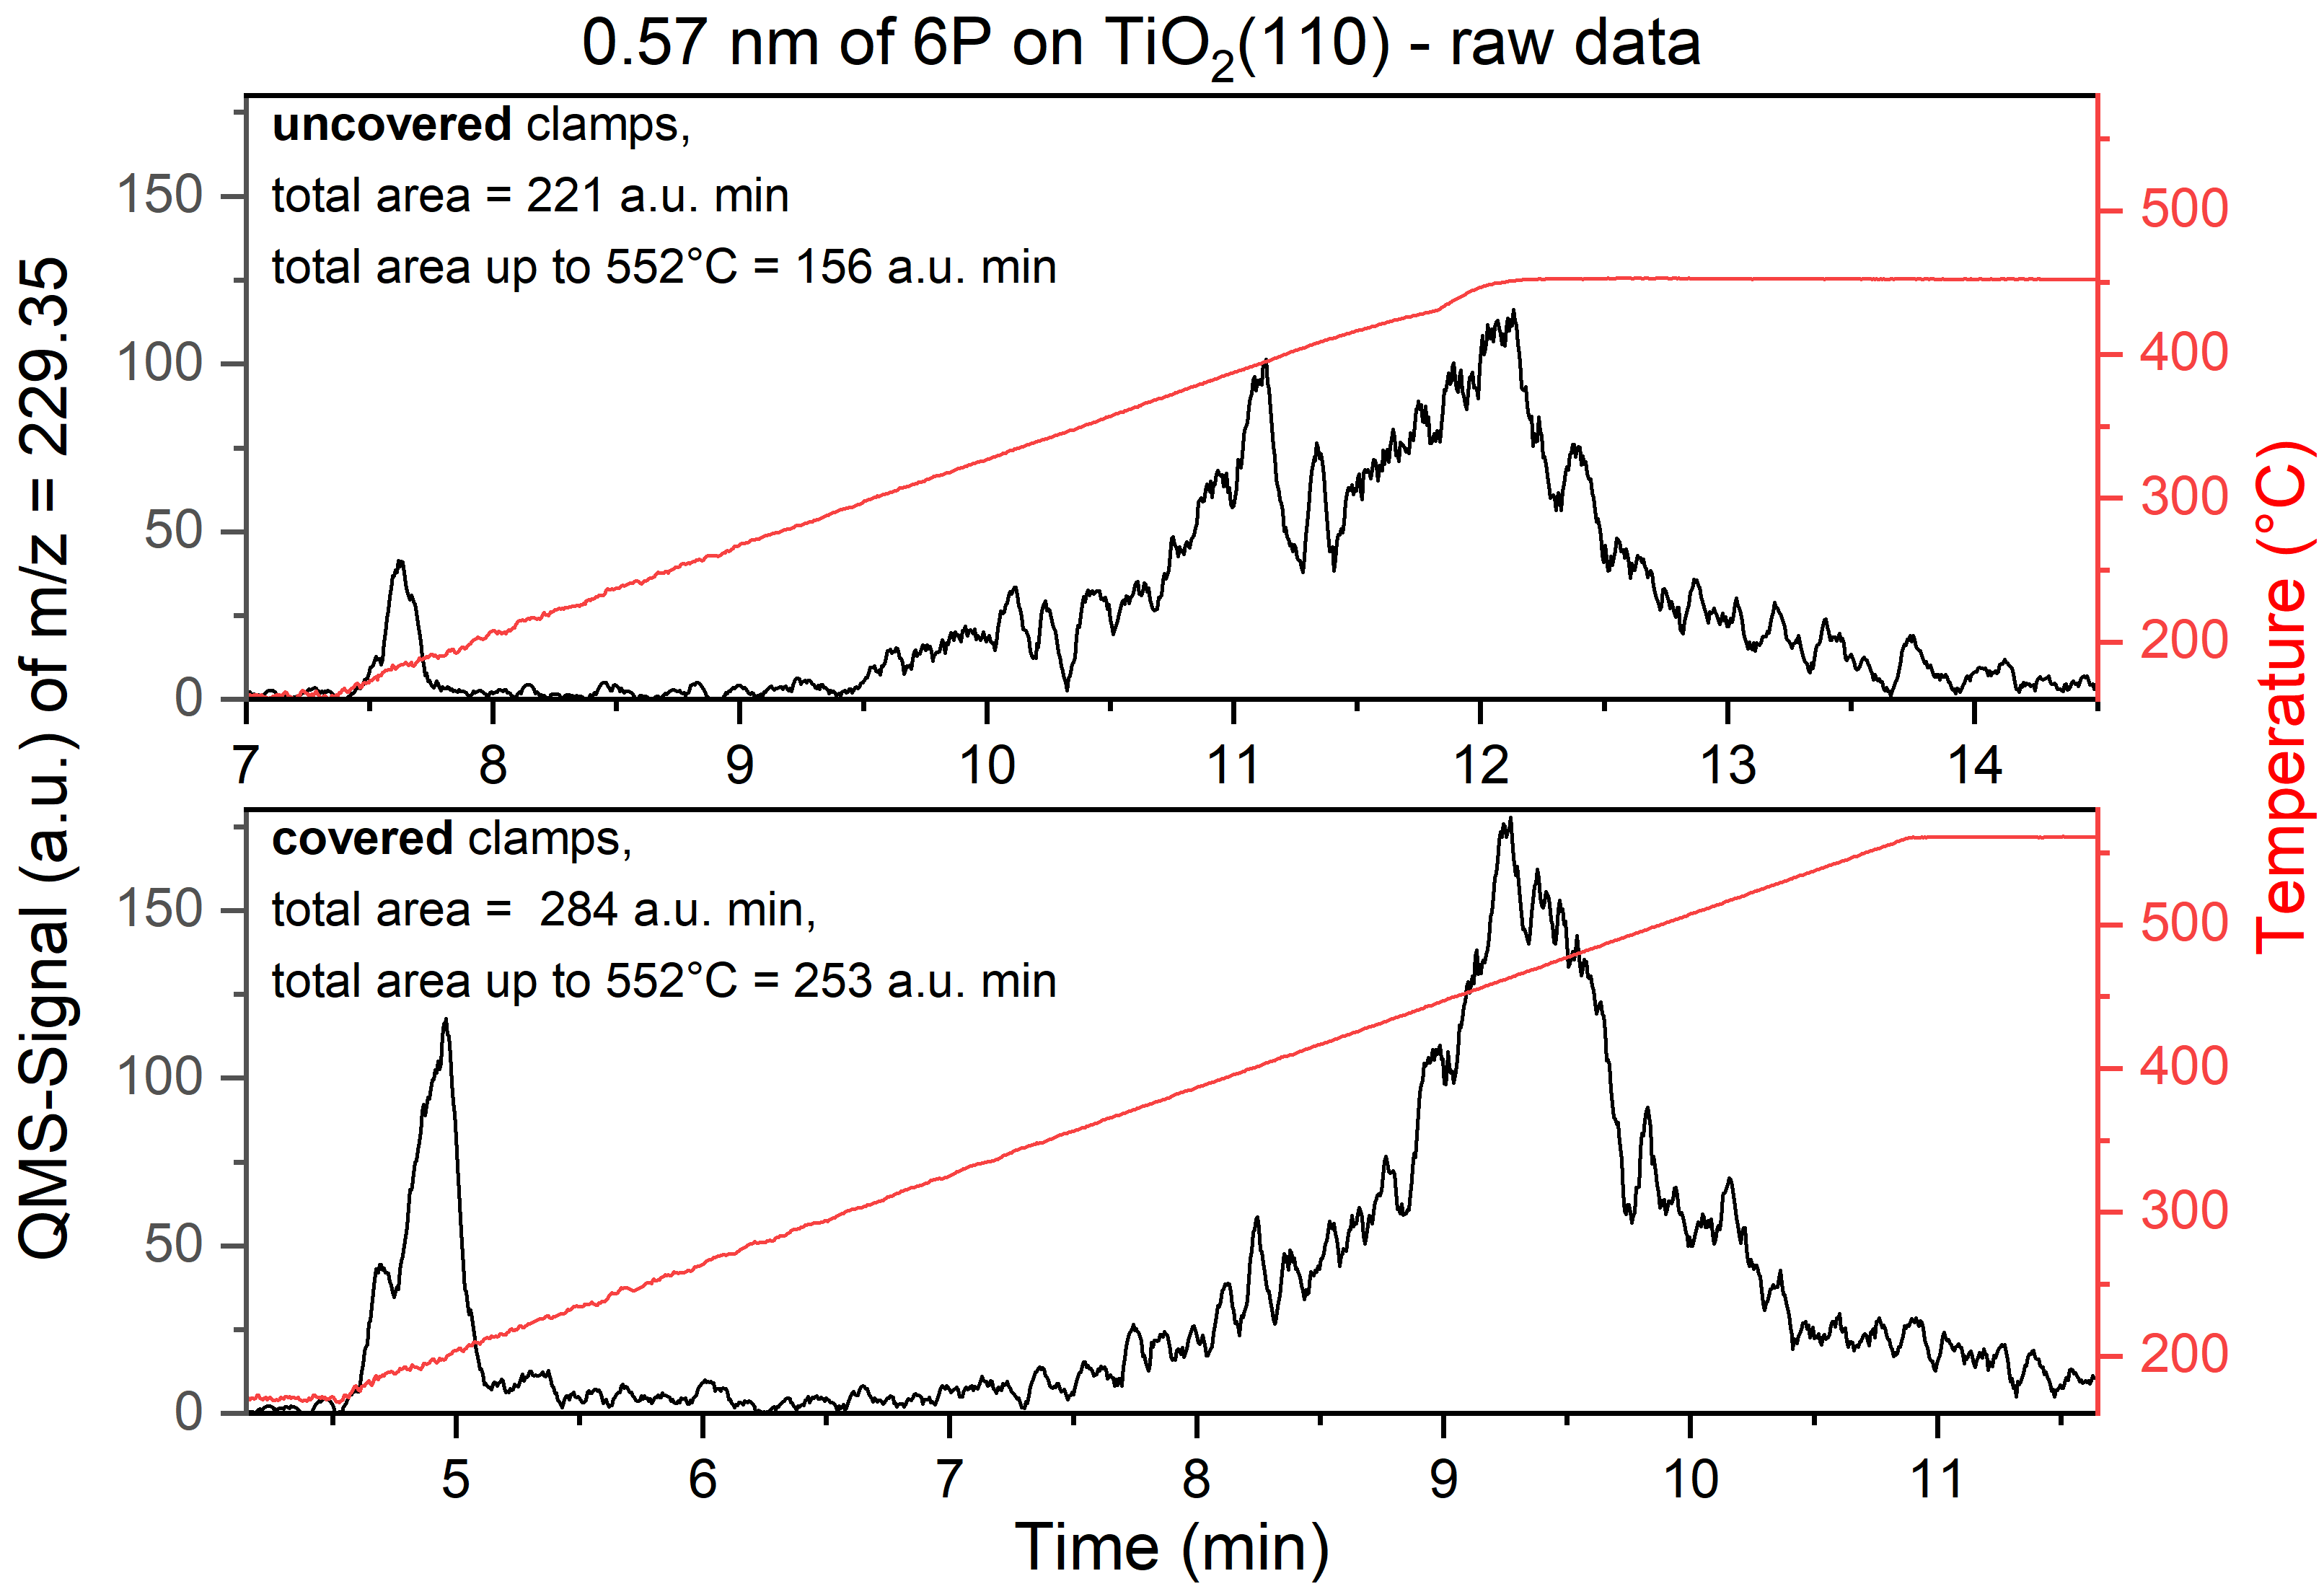
\includegraphics[width=9cm,height=8cm,keepaspectratio]{figures/results/some-graph.png}
	\setlength\belowcaptionskip{3pt}
	\caption{a) the first and b) second part.}
	\label{some-graph}
\end{figure}

Look at the Figure \ref{some-graph}!

\lipsum[70]


\subsection{Its second subsection}
\lipsum[77]



\section{Another section}

\lipsum[78]


\chapter{Conclusions}


\lipsum[55-59]




\clearpage
\phantomsection
\addcontentsline{toc}{chapter}{Bibliography}


%the bibliography style that you use
\bibliographystyle{ieeetr}

%the file which contains your references

\fancypagestyle{plain}{%
	\renewcommand{\headrulewidth}{0pt}%
	\fancyhf{}
	\fancyfoot[R]{\thepage}}
\bibliography{library.bib}

%It is good to have some appendix in your thesis - at least one


\clearpage
\phantomsection
\addcontentsline{toc}{chapter}{Appendix: Academic achievements}
\appendix
\chapter*{Appendix}

\lipsum[1]

\begin{itemize}
	\item Item number one, 
	\item item number two, 
	\item item number three, 
\end{itemize}

\lipsum[3]
\vspace{7pt}
\begin{table}[!h]
	\centering
	\ra{1.1}
	\caption{List of conferences at which I presented the results of investigations in the form of an oral presentation. }
	\label{conferences} 
	\vspace{-5pt}
	\begin{tabular}{@{}lp{0.12\linewidth}p{0.25\linewidth}p{0.45\linewidth}@{}}
		\doublerule
		Date             & Place               & Conference                                                                                     & Title of contribution                                                                                                                         \\ \midrule
		01.2026     & virtual   & A fancy Seminar                                                  & Really long name of the presentation \\
		06.2027     & virtual   &  Conference  number two                                               & something equally interesting               \\
		06.2029     & New York   & 11th International Conference                                                   & The same speech   \\
		06.2029     & Copenhagen   & Nanotechnology conference          & A revolutionary presentation       \\
		\bottomrule 
	\end{tabular}
\end{table}












\end{document}
